\documentclass[conference,a4paper]{IEEEtran}
\IEEEoverridecommandlockouts

\usepackage[T1]{fontenc}
\usepackage{cite}
\usepackage{amsmath,amssymb}
\usepackage{graphicx}
\usepackage{booktabs}
\usepackage{tabularx}
\usepackage[table]{xcolor}
\definecolor{coverhead}{RGB}{230,230,250}
\usepackage{listings}
\usepackage{tikz}
\usetikzlibrary{arrows.meta,positioning,calc}
\usepackage{pgfplots}
\pgfplotsset{compat=1.16}
\usepackage[hidelinks]{hyperref}

\graphicspath{{figures/}}
\newcolumntype{Y}{>{\raggedright\arraybackslash}X}

\lstset{
  basicstyle=\ttfamily\scriptsize,
  keywordstyle=\bfseries,
  commentstyle=\itshape,
  columns=fullflexible,
  keepspaces=true,
  breaklines=true,
  frame=lines,
  showstringspaces=false,
  xleftmargin=2pt,
  xrightmargin=2pt
}

\begin{document}

% ============================================================ cover page
\onecolumn
\thispagestyle{empty}
\begin{center}
\vspace*{1.6cm}

\includegraphics[width=0.5\textwidth]{mit_logo.png}\par
\vspace{1.1cm}
{\fontsize{15.8}{18}\selectfont\bfseries MANIPAL INSTITUTE OF TECHNOLOGY\par}
{\fontsize{10.5}{12.5}\selectfont (A Constituent Unit of Manipal Academy of Higher Education)\par}
\vspace{0.4cm}
{\fontsize{12.5}{15}\selectfont\bfseries School of Computer Engineering\par}
\vspace{0.9cm}
{\fontsize{12}{14}\selectfont\bfseries Foundations of Computer Vision Lab (CSE-3176)\par}
{\fontsize{11}{13}\selectfont Mini-Project Report\par}
\vspace{0.8cm}
{\fontsize{11}{13}\selectfont\itshape Project Title\par}
\vspace{0.6cm}
{\fontsize{15.5}{19}\selectfont\bfseries Vision-Assisted Survivor Localisation\\
in Maritime Search and Rescue\\
using Texture-Anomaly Modelling\par}
\vspace{0.9cm}
{\fontsize{11}{13}\selectfont\itshape Submitted by\par}
\vspace{0.35cm}
{\fontsize{10}{12}\selectfont
\arrayrulecolor{gray}
\renewcommand{\arraystretch}{1.45}
\begin{tabular}{|>{\centering\arraybackslash}p{7.2cm}|>{\centering\arraybackslash}p{2.2cm}|>{\centering\arraybackslash}p{3.4cm}|}
\hline
\rowcolor{coverhead}\textbf{Name} & \textbf{Roll No.} & \textbf{Registration No.} \\
\hline
Tanish Hemant Kuvar & 47 & 240962540 \\
\hline
M Vishal Kumar & 49 & 240962546 \\
\hline
Samyak Jain & & 240962638 \\
\hline
\end{tabular}
\arrayrulecolor{black}\par}
\vspace{0.9cm}
% {\fontsize{11}{13}\selectfont\itshape Under the guidance of\par}
% \vspace{0.2cm}
% {\fontsize{11}{13}\selectfont\bfseries Guide Name\par}
% \vspace{0.7cm}
{\fontsize{11.5}{14}\selectfont\bfseries Academic Year 2026--2027\par}
\end{center}
\twocolumn

% ============================================================ paper
\title{Vision-Assisted Survivor Localisation in Maritime Search and Rescue using Texture-Anomaly Modelling}

\author{
\IEEEauthorblockN{Tanish Hemant Kuvar}
\IEEEauthorblockA{Reg.\ No.\ 240962540\\
AIML, Section A}
\and
\IEEEauthorblockN{M. Vishal Kumar}
\IEEEauthorblockA{Reg.\ No.\ 240962546\\
AIML, Section A}
\and
\IEEEauthorblockN{Samyak Jain}
\IEEEauthorblockA{Reg.\ No.\ 240962638\\
AIML, Section A}
}

\maketitle

% ============================================================ abstract
\begin{abstract}
People in the water seen from a drone often cover fewer than 16 pixels, too few for appearance-based recognition. This paper presents a search-and-rescue (SAR) aid that models the water rather than the person. Each aerial RGB frame passes through six classical stages: illumination normalisation, Gabor and uniform local binary pattern (LBP) texture description, chi-square anomaly scoring against a robust local reference, glint suppression by chromaticity, morphological shape filtering, and temporal tracking. The output is a ranked shortlist of at most $k$ regions per frame, shown to an operator through a Tkinter desktop GUI and a browser-based console. No training data is required. On a synthetic benchmark of 6 sequences (360 frames, 739 annotated people), the system reaches 92.4\% recall@5 with 51.7\% precision and 1.77 false alarms per frame, rising to 99.3\% recall once the tracker has warmed up, at about 2.7 frames/s on a laptop CPU. An ablation shows that the temporal stage cuts false alarms by 35\%. These results validate the pipeline end to end; real-world performance remains to be measured on public datasets.
\end{abstract}

\begin{IEEEkeywords}
search and rescue, anomaly detection, Gabor filters, local binary patterns, morphological filtering, multi-frame tracking
\end{IEEEkeywords}

% ============================================================ introduction
\section{Introduction}

When a person falls overboard, a drone can cover a large area of sea quickly, but an operator watching the feed must find a head-sized target among waves, sun glint and foam. Learned detectors need large annotated datasets and can fail when the sea state, altitude or camera differs from training. This work instead treats survivor search as anomaly detection: it estimates what normal sea looks like in the current frame and reports regions that do not fit.

The contributions are:
\begin{enumerate}
  \item a six-stage pipeline built only from classical image processing operations, with no training step;
  \item a texture reference estimated per frame from a local median, which stays clean when targets are present;
  \item colour, shape and temporal tests that remove glint, foam and whitecaps;
  \item two operator front ends that expose every intermediate stage and parameter;
  \item an evaluation with recall@$k$, false alarms per frame and stage-by-stage ablation.
\end{enumerate}

% ============================================================ problem
\section{Problem Statement}

Given a sequence of daylight aerial RGB frames of open water, return for each frame a ranked list of at most $k$ regions likely to contain a person, each with a confidence value. Three properties make this hard:
\begin{itemize}
  \item \textit{Small targets:} 618 of the 739 annotated people in the benchmark measure under 16 px (square root of box area).
  \item \textit{Moving clutter:} waves, sun glint, whitecaps and debris all differ from calm water and change from frame to frame.
  \item \textit{No fixed appearance:} a partly submerged person may show only a head, and clothing colour varies.
\end{itemize}

\subsection{System Requirements}

Table~\ref{tab:requirements} lists the requirements and how the system meets them.

\begin{table}[!t]
\centering
\footnotesize
\caption{System Requirements}
\label{tab:requirements}
\begin{tabularx}{\columnwidth}{@{}lYY@{}}
\toprule
Type & Requirement & How it is met \\
\midrule
Functional & Accept video, an image folder or an image & \texttt{run} command and GUI loaders \\
Functional & Output a ranked top-$k$ list as overlay and CSV & \texttt{run -{}-output -{}-csv}; shortlist panels \\
Functional & Inspect stages and tune parameters & Stage selector, 16 sliders, JSON configs \\
Functional & Provide a GUI front end & Tkinter GUI and browser console \\
Functional & Evaluate on annotated data & \texttt{evaluate}; COCO and YOLO loaders \\
Non-funct. & Run on a CPU, no GPU & $\approx$2.7 frames/s at $1280\times720$ \\
Non-funct. & Repeatable and tested & 40 passing unit and integration tests \\
Software & Python, NumPy $\geq$1.24, OpenCV $\geq$4.8, Pillow, Matplotlib, pytest, Tkinter & \texttt{requirements.txt} \\
Input & Daylight aerial RGB of open water & Night and thermal out of scope \\
\bottomrule
\end{tabularx}
\end{table}

% ============================================================ methodology
\section{Methodology}

Stages 1 to 5 run on each frame independently; stage 6 uses the history across frames. Fig.~\ref{fig:pipeline} shows the data flow.

\begin{figure*}[!t]
\centering
\resizebox{\textwidth}{!}{%
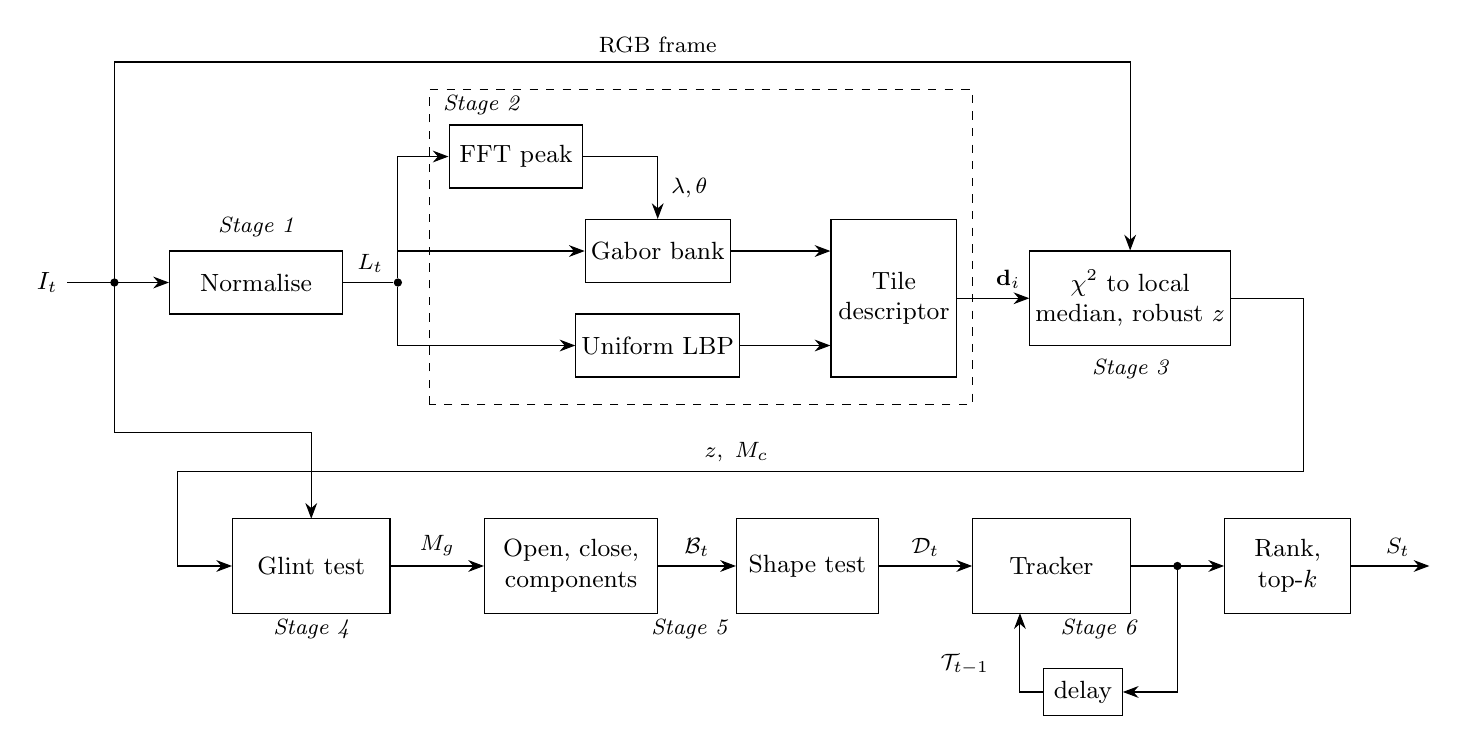
\begin{tikzpicture}[
  >={Stealth[length=2mm]},
  line width=0.4pt,
  every node/.style={font=\small},
  blk/.style={draw,rectangle,minimum height=8mm,align=center,inner sep=2pt},
  sig/.style={font=\footnotesize},
  stg/.style={font=\footnotesize\itshape},
  dot/.style={circle,fill,inner sep=0pt,minimum size=3pt}
]
\node[blk,minimum width=22mm] (norm) at (1.9,0) {Normalise};
\node[dot] (split) at (3.7,0) {};
\node[blk,minimum width=17mm] (fft) at (5.2,1.6) {FFT peak};
\node[blk,minimum width=18mm] (gabor) at (7,0.4) {Gabor bank};
\node[blk,minimum width=18mm] (lbp) at (7,-0.8) {Uniform LBP};
\node[blk,minimum width=16mm,minimum height=20mm] (tile) at (10,-0.2) {Tile\\descriptor};
\node[blk,minimum width=22mm,minimum height=12mm] (chi) at (13,-0.2) {$\chi^2$ to local\\median, robust $z$};
\draw[dashed] (4.1,-1.55) rectangle (11.0,2.45);
\node[stg,anchor=west] at (4.15,2.25) {Stage 2};
\node[stg] at (1.9,0.7) {Stage 1};
\node[stg] at (13,-1.1) {Stage 3};
\node[anchor=east] (inp) at (-0.5,0) {$I_t$};
\draw[->] (-0.5,0) -- (norm.west);
\node[dot] at (0.1,0) {};
\draw[->] (0.1,0) -- (0.1,2.8) -- (13,2.8) -- (chi.north);
\node[sig,above] at (7,2.8) {RGB frame};
\draw[->] (0.1,0) -- (0.1,-1.9) -- (2.6,-1.9) -- (2.6,-3.0);
\draw (norm.east) -- (split);
\node[sig,above] at (3.35,0) {$L_t$};
\draw[->] (split) |- (fft.west);
\draw[->] (split) |- (gabor.west);
\draw[->] (split) |- (lbp.west);
\draw[->] (fft.east) -| (gabor.north);
\node[sig,anchor=west] at (7.05,1.2) {$\lambda,\theta$};
\draw[->] (gabor.east) -- (gabor.east -| tile.west);
\draw[->] (lbp.east) -- (lbp.east -| tile.west);
\draw[->] (tile.east) -- (chi.west);
\node[sig,above] at (11.45,-0.2) {$\mathbf{d}_i$};
\node[blk,minimum width=20mm,minimum height=12mm] (glint) at (2.6,-3.6) {Glint test};
\node[blk,minimum width=22mm,minimum height=12mm] (morph) at (5.9,-3.6) {Open, close,\\components};
\node[blk,minimum width=18mm,minimum height=12mm] (shape) at (8.9,-3.6) {Shape test};
\node[blk,minimum width=20mm,minimum height=12mm] (track) at (12,-3.6) {Tracker};
\node[blk,minimum width=16mm,minimum height=12mm] (rank) at (15,-3.6) {Rank,\\top-$k$};
\node[blk,minimum width=10mm,minimum height=6mm] (delay) at (12.4,-5.2) {delay};
\draw[->] (chi.east) -- (15.2,-0.2) -- (15.2,-2.4) -- (0.9,-2.4) -- (0.9,-3.6) -- (glint.west);
\node[sig,above] at (8,-2.4) {$z,\ M_c$};
\draw[->] (glint.east) -- (morph.west);
\node[sig,above] at (4.2,-3.6) {$M_g$};
\draw[->] (morph.east) -- (shape.west);
\node[sig,above] at (7.5,-3.6) {$\mathcal{B}_t$};
\draw[->] (shape.east) -- (track.west);
\node[sig,above] at (10.4,-3.6) {$\mathcal{D}_t$};
\draw[->] (track.east) -- (rank.west);
\node[dot] at (13.6,-3.6) {};
\draw[->] (13.6,-3.6) -- (13.6,-5.2) -- (delay.east);
\draw[->] (delay.west) -- (11.6,-5.2) -- (11.6,-4.2);
\node[sig,below] at (10.9,-4.6) {$\mathcal{T}_{t-1}$};
\draw[->] (rank.east) -- (16.8,-3.6);
\node[sig,above] at (16.4,-3.6) {$S_t$};
\node[stg] at (2.6,-4.4) {Stage 4};
\node[stg] at (7.4,-4.4) {Stage 5};
\node[stg] at (12.6,-4.4) {Stage 6};
\end{tikzpicture}%
}
\caption{Block diagram of the pipeline. $I_t$: input frame; $L_t$: normalised lightness; $\lambda,\theta$: dominant wavelength and orientation; $\mathbf{d}_i$: descriptor of tile $i$; $z$: anomaly map; $M_c$, $M_g$: candidate mask before and after the glint test; $\mathcal{B}_t$: blobs; $\mathcal{D}_t$: detections; $\mathcal{T}_{t-1}$: previous tracks; $S_t$: shortlist.}
\label{fig:pipeline}
\end{figure*}

The filtering operations of stages 1, 2, 4 and 5 are detailed in Section~\ref{sec:enhancement}. This section describes how they combine into a decision.

\subsection{Tile Descriptors}

The normalised lightness is divided into overlapping square tiles of side $T$ with stride $T/2$, so a person on a tile border is not split. With automatic sizing, $T$ is about twice the expected person size: 32 px at 1920 px frame width, scaled with frame width and limited to 16--64 px. Each tile descriptor holds the mean Gabor energy of every filter and the normalised 59-bin uniform LBP histogram~\cite{ojala}.

\subsection{Anomaly Scoring (Stage 3)}

The reference for normal sea is the median descriptor over $9\times9$-tile windows, interpolated back to every tile. A median stays clean when a person or a boat covers some tiles, and the local window adapts to near and far field. Each tile is compared with its reference by the chi-square distance, computed separately for LBP and for reference-normalised Gabor energy:
\begin{equation}
\chi^2(\mathbf{a}, \mathbf{b}) = \frac{1}{2} \sum_i \frac{(a_i - b_i)^2}{a_i + b_i}.
\end{equation}
The two distances are put on one scale with a robust z-score and averaged with equal weight:
\begin{equation}
z = \frac{d - \operatorname{median}(d)}{1.4826 \cdot \operatorname{MAD}(d)}.
\end{equation}
The median absolute deviation (MAD) is used because targets are outliers that would inflate a standard deviation. Each pixel takes the maximum $z$ of the tiles covering it, and the anomalous region is $z > 3$. Inside it, candidate pixels are those whose Lab colour differs from a median-filtered local sea colour by more than $\operatorname{median} + 4\sigma_{\mathrm{MAD}}$, which turns a coarse tile into a pixel-accurate blob.

\subsection{Temporal Association and Ranking (Stage 6)}

Detections are linked between frames by greedy nearest neighbour around a constant-velocity prediction within a 40 px radius. A track is promoted after 5 hits if its drift is coherent:
\begin{equation}
c = \exp\!\left(-\frac{s}{6\,\mathrm{px}}\right) \geq 0.25,
\end{equation}
where $s$ is the RMS deviation of the step velocities from their mean. Gaps of up to 3 frames are tolerated, covering a head briefly under a wave. Optional camera-motion compensation estimates the frame-to-frame translation by phase correlation. Promoted tracks are ranked by
\begin{equation}
\mathrm{conf} = 0.4\,\mathrm{conf}_{\mathrm{anom}} + 0.6\,\frac{\min(h, 10)}{10}\,c,
\end{equation}
where $h$ is the number of hits and $\mathrm{conf}_{\mathrm{anom}}$ an exponential moving average of the blob confidence; the result is multiplied by 0.8 per missed frame. The top $k$ tracks form the shortlist.

% ============================================================ enhancement
\section{Image Enhancement and Filtering Techniques}
\label{sec:enhancement}

Every stage uses classical intensity, spatial, frequency or morphological operations~\cite{gonzalez,szeliski,sonka}, implemented with OpenCV~\cite{howse,baggio,laganiere} and listed here in pipeline order.

\subsection{Illumination Normalisation (Stage 1)}

Three steps run on the Lab lightness channel so that texture statistics are comparable across the frame:
\begin{enumerate}
  \item \textit{Flat-fielding:} lightness is divided by a heavily Gaussian-smoothed copy of itself ($\sigma$ = 1/8 of frame width), removing the sun-side and far-field brightness gradient.
  \item \textit{CLAHE:} contrast-limited adaptive histogram equalisation with clip limit 2.0 over $8\times8$ regions.
  \item \textit{Piecewise-linear stretch:} a three-segment transform maps the 1st and 99th percentiles to 10 and 245, so a few glint pixels do not compress the rest.
\end{enumerate}
Fig.~\ref{fig:norm} shows that the brightness gradient disappears while wave texture is kept.

\begin{figure}[!t]
\centering
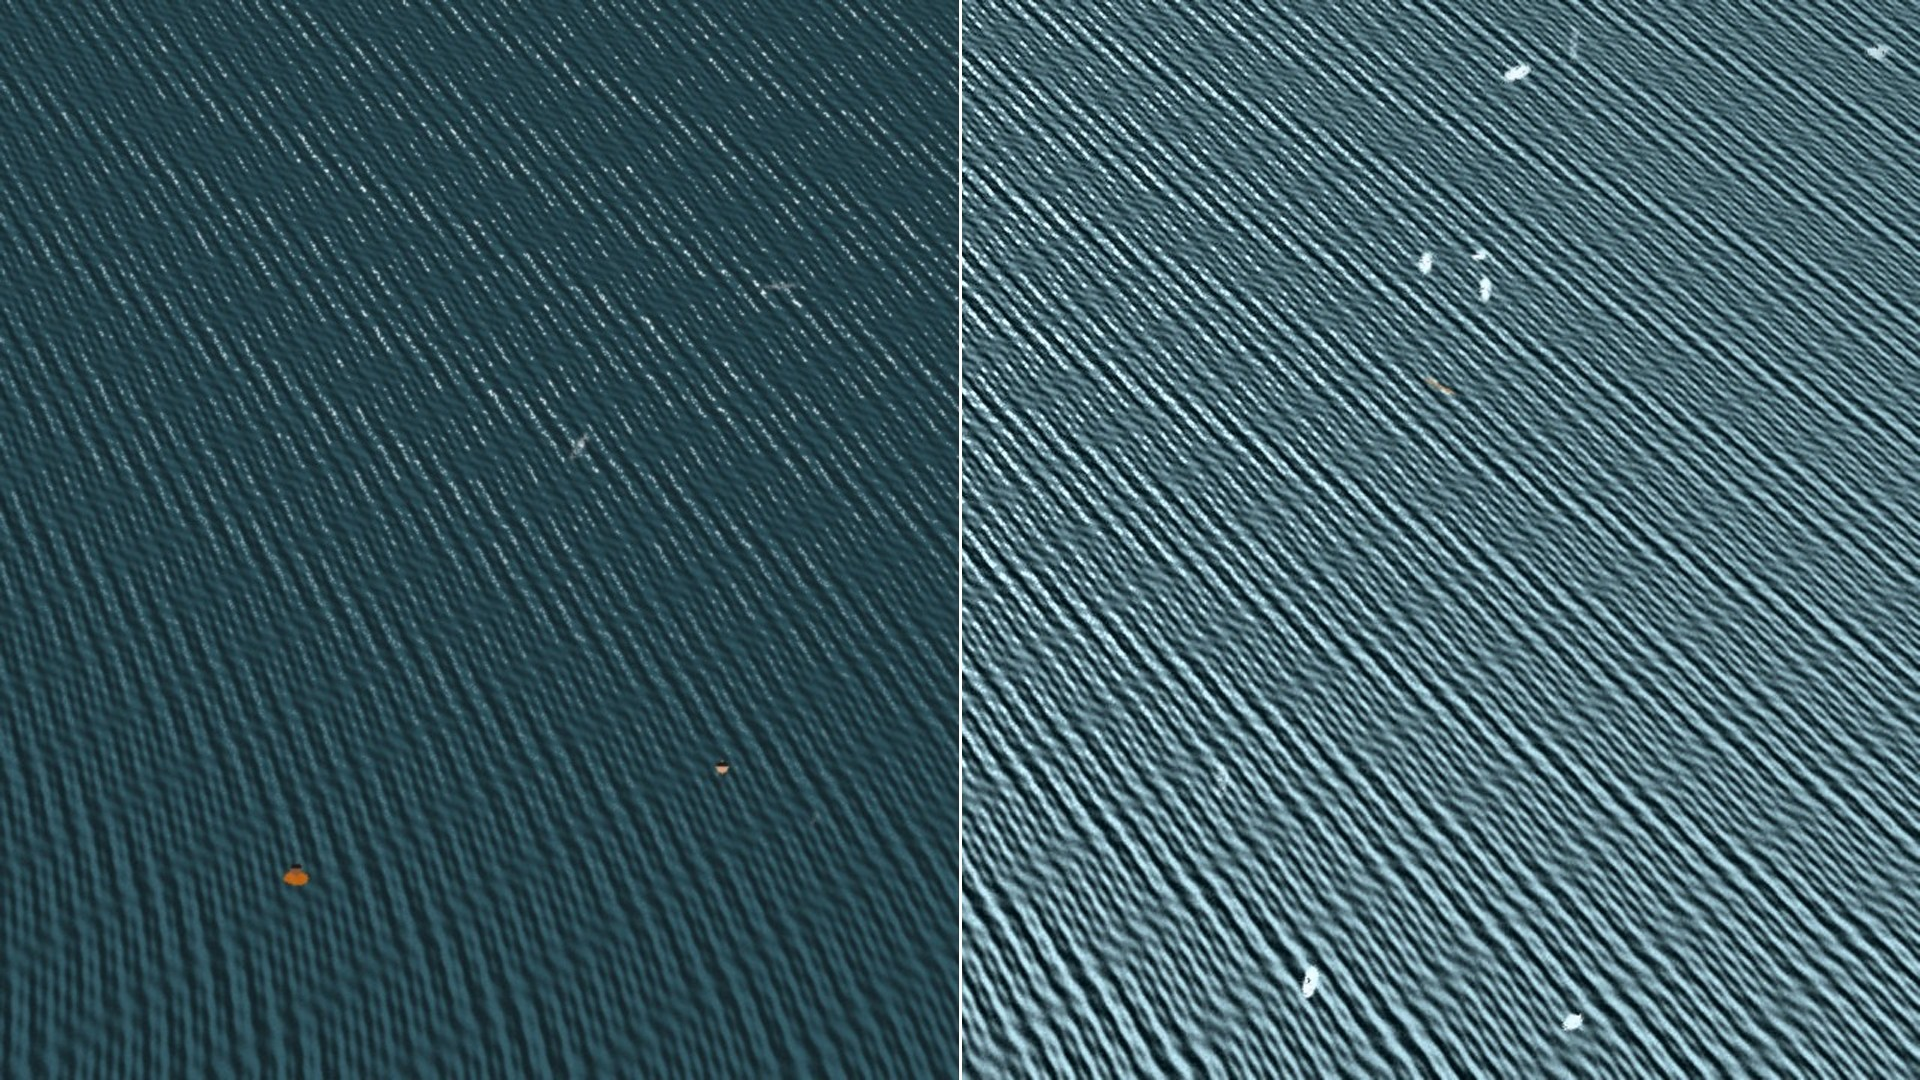
\includegraphics[width=\columnwidth]{norm_split.jpg}
\caption{A frame before (left) and after (right) normalisation.}
\label{fig:norm}
\end{figure}

\subsection{Frequency-Domain Wave Estimate}

The frame is split into far, middle and near bands. For each band, the 2-D DFT of a Hann-windowed patch gives a power spectrum, and its strongest peak with a wavelength of 4--32 px gives the dominant wavelength $\lambda$ and orientation $\theta$. This tunes the Gabor bank to the waves actually present.

\subsection{Gabor Filtering}

For each band wavelength the bank has four orientations, $\theta$, $\theta+45^\circ$, $\theta+90^\circ$ and $\theta+135^\circ$, with $\sigma = 0.56\lambda$ and aspect ratio $\gamma = 0.5$. Each filter is applied as an even and odd pair, and the local energy $\sqrt{e^2 + o^2}$ is used because it does not depend on wave phase. Long-wavelength filters run on a downsampled image at no loss in tile averages. Fig.~\ref{fig:kernels} shows the even kernels of one wavelength.

\begin{figure}[!t]
\centering

\includegraphics[width=\columnwidth]{kernels.png}
\caption{Even Gabor kernels at the four orientations of one wavelength.}
\label{fig:kernels}
\end{figure}

\subsection{Uniform Local Binary Patterns}

Each pixel is compared with its eight neighbours (bit = 1 if neighbour $\geq$ centre), and the code is mapped to one of 59 uniform bins~\cite{ojala}. The per-tile histogram describes micro-texture independent of absolute brightness.

\subsection{Median Filtering and Colour Distance}

A median-filtered copy of the frame gives the local sea colour while ignoring small objects. Distances to it are measured in Lab space.

\subsection{Glint Suppression by Chromaticity (Stage 4)}

Specular glint saturates all channels together, so its rgb chromaticity $(R,G,B)/(R+G+B)$ lies close to $(\frac13,\frac13,\frac13)$. A pixel is glint if its mean is at least $0.8 \cdot 255$ and its chromaticity distance from grey is at most 0.06. Requiring both conditions keeps dark, colourless targets such as a black wetsuit.

\subsection{Morphological Filtering (Stage 5)}

Opening with a $3\times3$ ellipse removes specks and closing with a $5\times5$ ellipse joins the fragments of a partly submerged body. Connected components (8-connectivity) must have an area of 12--2500 px, eccentricity $\leq 0.97$ from second-order moments (rejecting foam streaks) and solidity, the ratio of area to convex-hull area, $\geq 0.45$ (rejecting ragged foam). Each blob is scored $s$ = peak tile $z$ $\times$ mean colour contrast, with confidence $s/(s+50)$. Fig.~\ref{fig:morph} shows kept and rejected blobs.

\begin{figure}[!t]
\centering
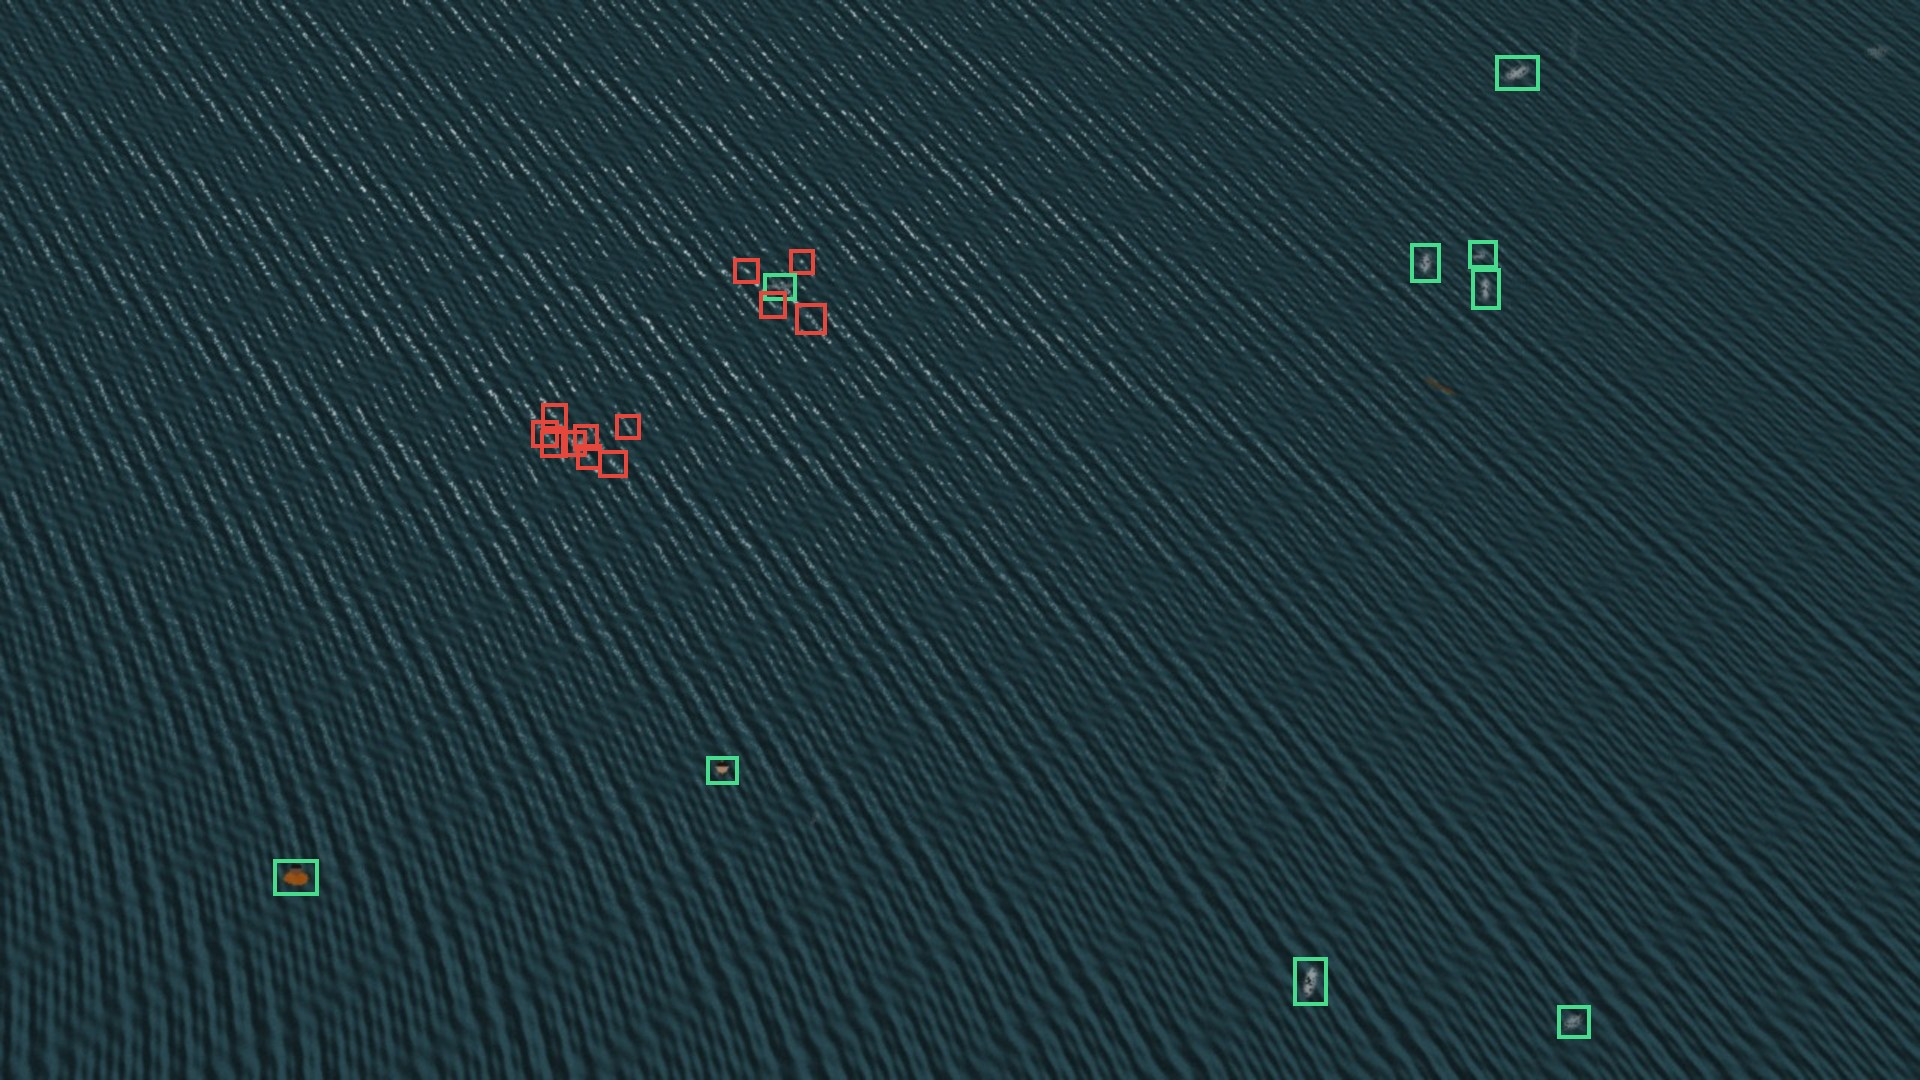
\includegraphics[width=\columnwidth]{morph_blobs.jpg}
\caption{Blobs after morphology: green passed the shape filter, red were rejected.}
\label{fig:morph}
\end{figure}

\subsection{Mapping to Lab Sessions 1--5}

Table~\ref{tab:labs} maps each technique to the function that implements it.

\begin{table}[!t]
\centering
\footnotesize
\caption{Lab Techniques and Their Implementation}
\label{tab:labs}
\begin{tabularx}{\columnwidth}{@{}Y>{\raggedright\arraybackslash}p{0.55\columnwidth}@{}}
\toprule
Technique & Implemented in \\
\midrule
Intensity transform: piecewise-linear stretch & \texttt{normalise.piecewise\_linear} \\
Histogram processing: CLAHE & \texttt{normalise.normalise} \\
Spatial filtering: Gaussian, median, Gabor convolution & \texttt{normalise.flat\_field}, \texttt{anomaly.colour\_deviation}, \texttt{texture.gabor\_energy} \\
Frequency domain: 2-D DFT, phase correlation & \texttt{texture.estimate\_wave}, \texttt{pipeline.estimate\_shift} \\
Texture: uniform LBP, chi-square distance & \texttt{texture.uniform\_lbp}, \texttt{anomaly.chi\_square} \\
Colour spaces: Lab, rgb chromaticity & \texttt{anomaly.colour\_deviation}, \texttt{glint.chromaticity} \\
Thresholding: median $+\,k\cdot$MAD & \texttt{anomaly.score\_anomalies} \\
Morphology: opening, closing & \texttt{morphology.refine} \\
Components, moments, convex hull & \texttt{morphology.refine}, \texttt{eccentricity}, \texttt{solidity} \\
\bottomrule
\end{tabularx}
\end{table}

% ============================================================ UI
\section{UI Design}

Two front ends run the same pipeline and share one configuration. The Tkinter desktop GUI suits inspecting and tuning a single frame; the browser console analyses a whole sequence and plays it back, which suits a live demonstration.

\subsection{Desktop GUI}

The desktop GUI (Fig.~\ref{fig:gui}) places the frame in the centre, input, playback, stage selection, parameters and export on the left, and the ranked shortlist with frame diagnostics on the right. The display-stage dropdown shows any of ten views, from the input to the final overlay. For the frame shown, the diagnostics report 321 of 6254 tiles anomalous and 9 of 26 blobs kept, with 3 tracks on the shortlist.

\begin{figure}[!t]
\centering
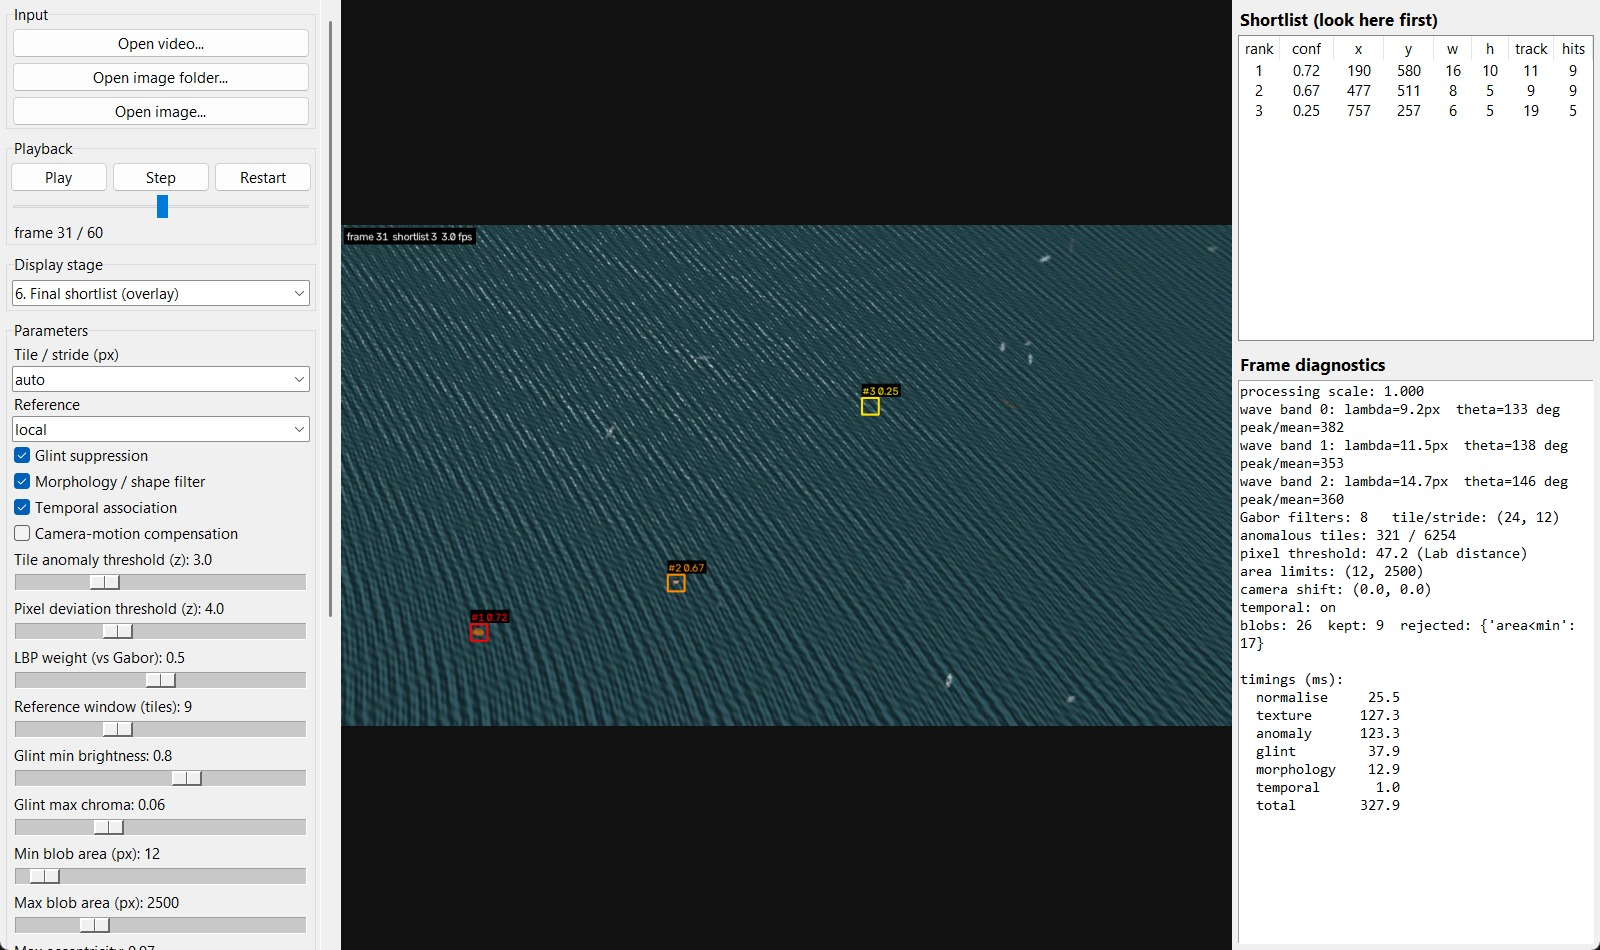
\includegraphics[width=\columnwidth]{gui.jpg}
\caption{Desktop GUI on sequence 5, frame 31. The shortlist table gives rank, confidence, box, track id and hits.}
\label{fig:gui}
\end{figure}

\subsection{Web Operator Console}

The console (Fig.~\ref{fig:web}) is started with \texttt{python -m sarvision web} and served at \texttt{localhost:8765} by a standard-library HTTP server. Stages 1--5 run in parallel on a thread pool while stage 6 runs in order, and the browser plays the result back at the source frame rate as the timeline fills in. The header shows sequence-level recall, precision, false alarms and throughput; the right panel shows ranked shortlist cards with crops, frame telemetry (wave-spectrum dial, per-stage timings, tile and blob counts) and tuning controls with ablation presets. A stage strip under the timeline opens any intermediate result for the current frame.

\begin{figure*}[!t]
\centering
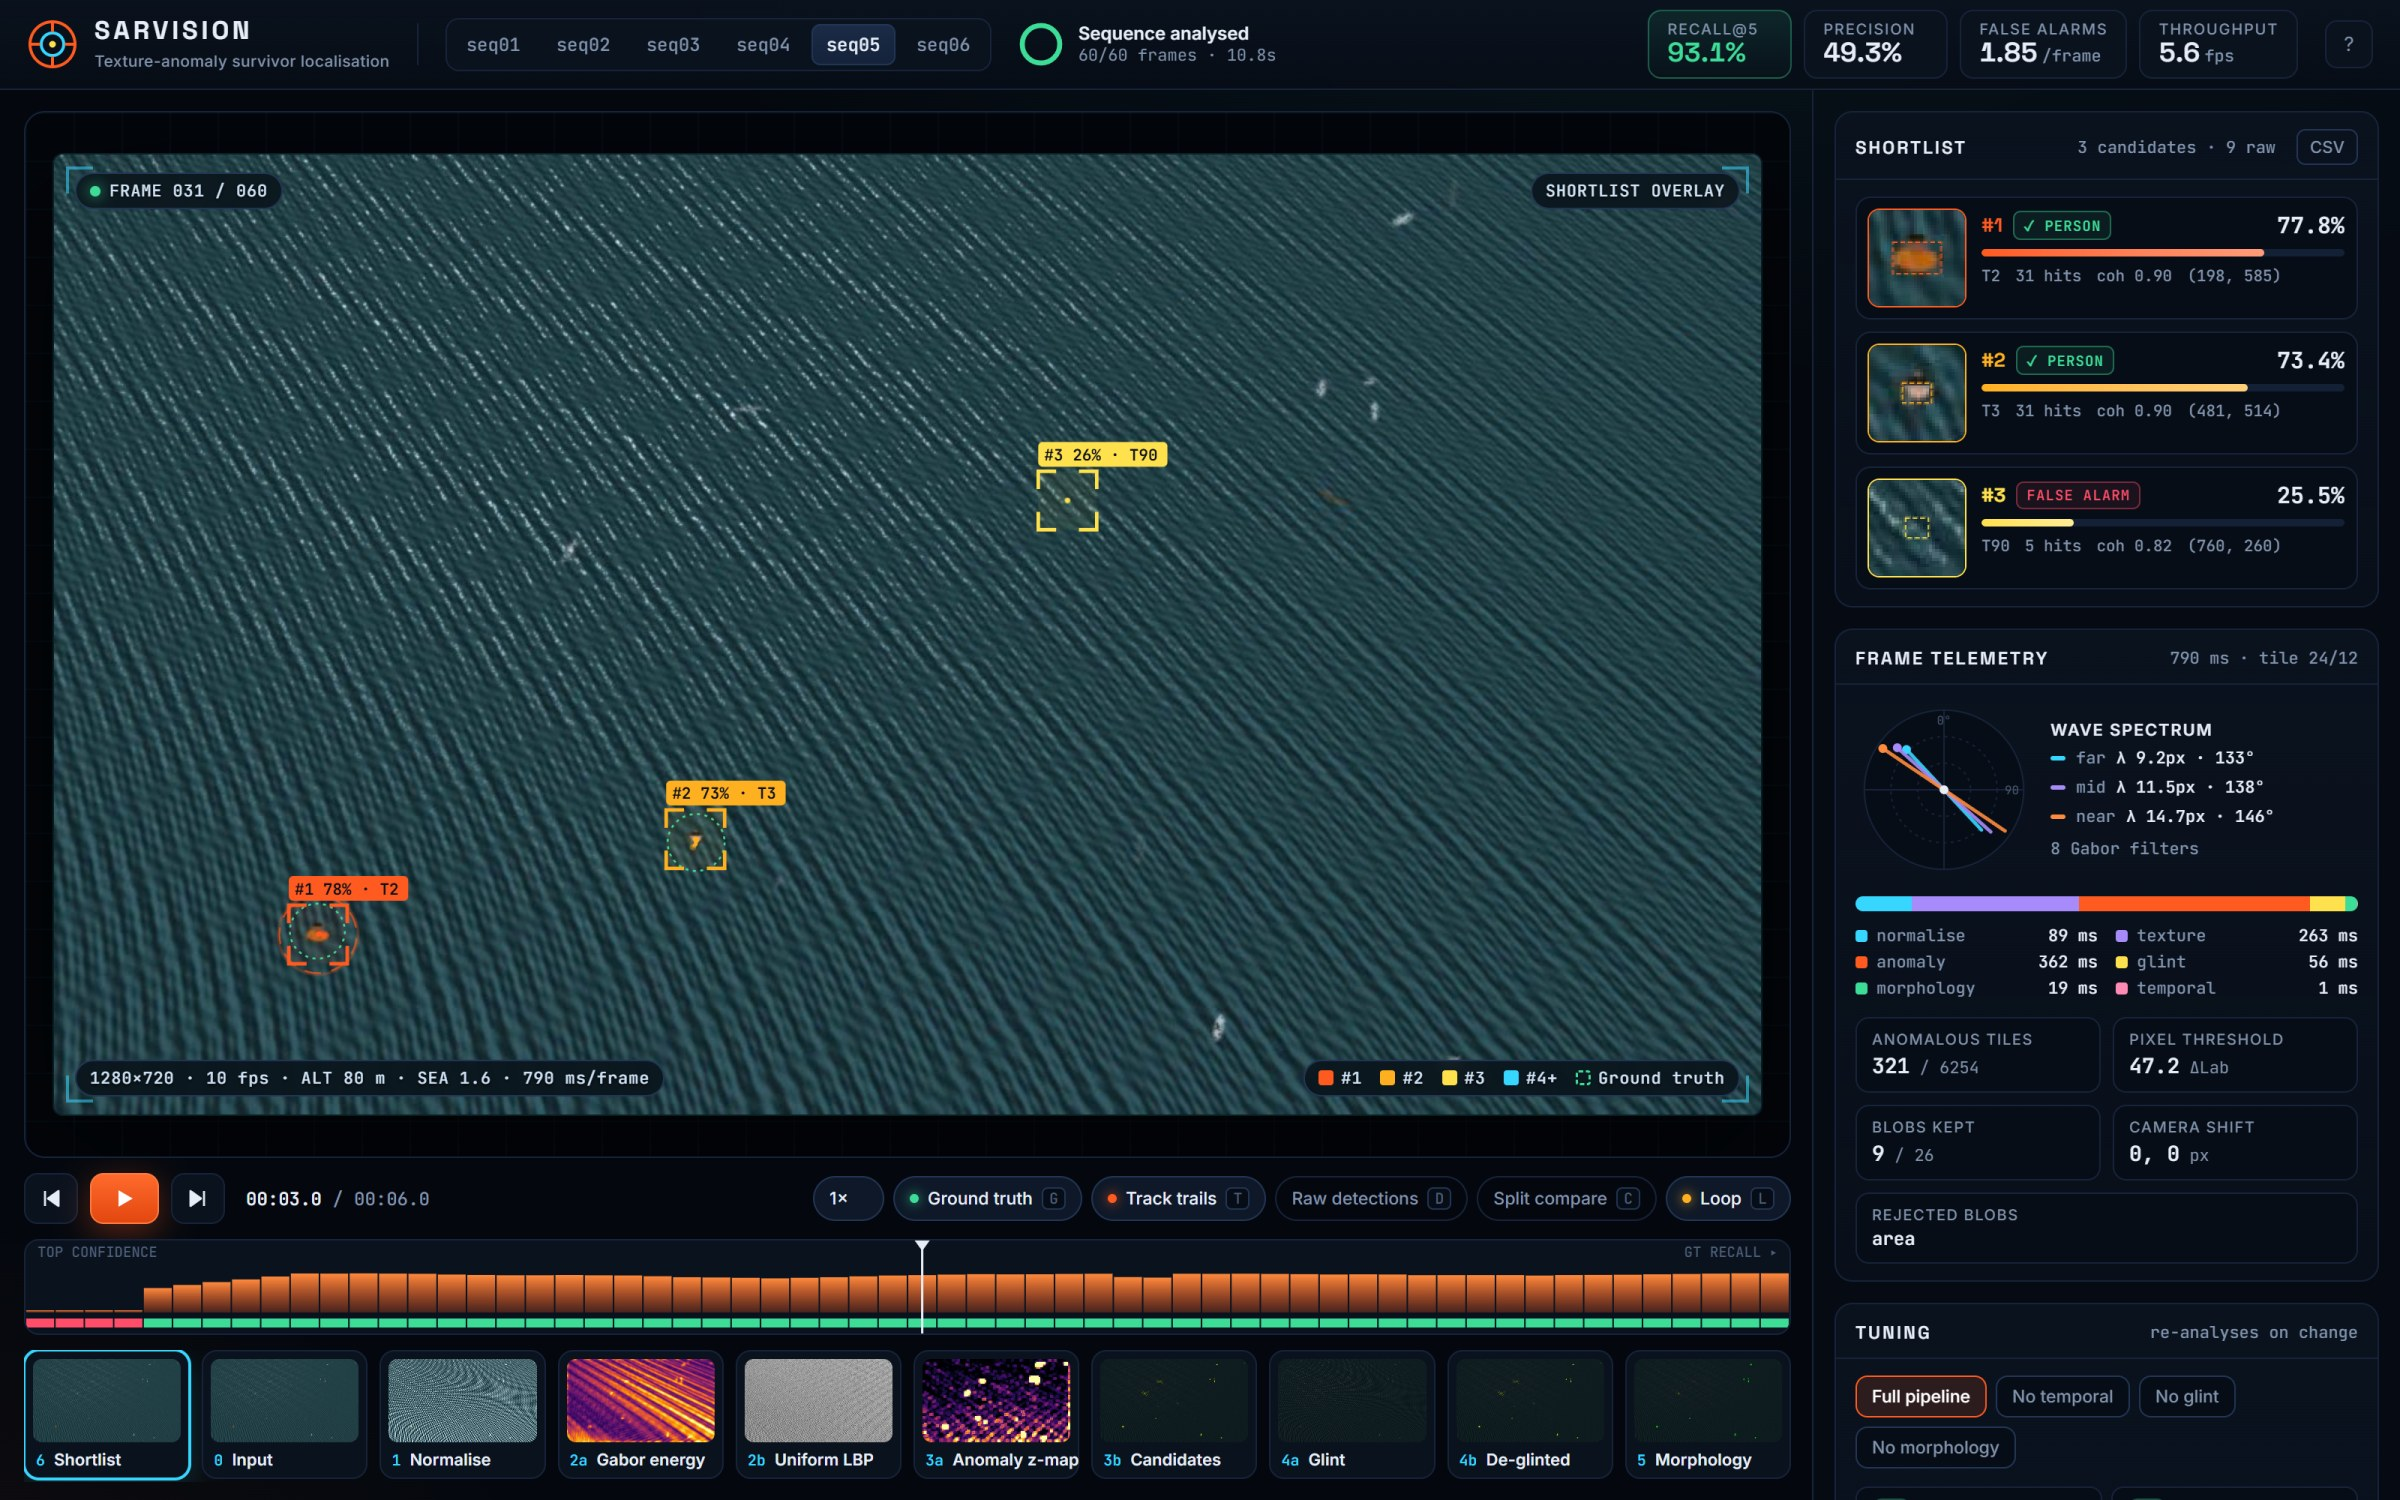
\includegraphics[width=0.9\textwidth]{web_console.jpg}
\caption{Web console on sequence 5, frame 31. Two people are ranked \#1 and \#2 (77.8\% and 73.4\%); \#3 is a short-lived false alarm (25.5\%). Telemetry shows dominant wavelengths of 9.2, 11.5 and 14.7 px in the far, middle and near bands.}
\label{fig:web}
\end{figure*}

% ============================================================ implementation
\section{VS Code for Functional Design}

The system is a Python package, \texttt{sarvision}, of about 2900 lines developed in VS Code, with one module per stage and one shared configuration dataclass so the GUIs, command line and evaluation run identical code (Table~\ref{tab:modules}).

\begin{table}[!t]
\centering
\footnotesize
\caption{Modules of the \texttt{sarvision} Package}
\label{tab:modules}
\begin{tabularx}{\columnwidth}{@{}>{\raggedright\arraybackslash}p{0.33\columnwidth}Y@{}}
\toprule
File & Responsibility \\
\midrule
\texttt{config.py} & All tunable parameters \\
\texttt{normalise.py} & Stage 1: flat-field, CLAHE, stretch \\
\texttt{texture.py} & Stage 2: DFT, Gabor bank, LBP, tiles \\
\texttt{anomaly.py} & Stage 3: reference, $\chi^2$, robust $z$ \\
\texttt{glint.py} & Stage 4: chromaticity glint test \\
\texttt{morphology.py} & Stage 5: morphology, shape filter \\
\texttt{tracking.py} & Stage 6: association, ranking \\
\texttt{pipeline.py} & Stage order; motion compensation \\
\texttt{gui.py}, \texttt{viz.py} & Tkinter GUI; stage rendering \\
\texttt{web/} & Browser console server and page \\
\texttt{cli.py} & Command-line entry point \\
\texttt{datasets.py},\newline \texttt{metrics.py},\newline \texttt{evaluate.py} & Loaders, metrics, ablations \\
\texttt{synthetic.py} & Synthetic benchmark generator \\
\bottomrule
\end{tabularx}
\end{table}

The application is run as follows:
\begin{lstlisting}[language=bash]
pip install -r requirements.txt
python -m sarvision synth --out data/synthetic
python -m sarvision gui data/synthetic/seq02.mp4
python -m sarvision web data/synthetic/seq05.mp4
python -m sarvision run --input data/synthetic/seq02.mp4 \
    --output out.mp4 --csv shortlist.csv
python -m sarvision evaluate --coco data/synthetic/annotations.json \
    --ablations full,no_temporal,no_glint,no_morphology
\end{lstlisting}

The core of stages 2 and 3 is shown below.
\begin{lstlisting}[language=Python]
def gabor_energy(gray, filt):
    f = gray.astype(np.float32)
    e = cv2.filter2D(f, cv2.CV_32F, filt.even,
                     borderType=cv2.BORDER_REFLECT)
    o = cv2.filter2D(f, cv2.CV_32F, filt.odd,
                     borderType=cv2.BORDER_REFLECT)
    return cv2.magnitude(e, o)   # sqrt(e^2 + o^2)

def chi_square(a, b):
    return 0.5 * np.sum((a - b) ** 2 / (a + b + EPS),
                        axis=-1)

def robust_z(x):
    med = np.median(x)
    mad = np.median(np.abs(x - med)) * MAD_TO_SIGMA
    if mad < EPS:
        mad = x.std() + EPS
    return (x - med) / mad
\end{lstlisting}

% ============================================================ results
\section{Results and Discussion}

\subsection{Evaluation Protocol}

The benchmark has 6 rendered sequences of 60 frames at $1280\times720$ and 10 fps with 739 annotated people, covering altitudes of 50--150 m, calm to rough sea, strong glitter, a dark-clothed person and a panning camera. A prediction is a hit when its centre lies within $\max(8\,\mathrm{px}, \max(w,h))$ of the ground-truth centre, since IoU is too harsh for 10--30 px boxes. Steady-state figures exclude the first 4 frames of each sequence, before the tracker can promote any track. \textit{All results are synthetic}: they validate the pipeline and evaluation, not real-world performance.

\subsection{Ablation}

Table~\ref{tab:ablation} compares the full system with one stage switched off at a time.

\begin{table*}[!t]
\centering
\footnotesize
\caption{Ablation on the Synthetic Benchmark at $k = 5$ (FA: false alarms; SS: steady state)}
\label{tab:ablation}
\begin{tabular}{@{}lrrrrrr@{}}
\toprule
Run & Recall@5 & Precision@5 & FA/frame & SS recall@5 & SS FA/frame & Frames/s \\
\midrule
\textbf{Full system} & \textbf{92.4\%} & \textbf{51.7\%} & \textbf{1.77} & \textbf{99.3\%} & \textbf{1.90} & \textbf{2.67} \\
Without temporal stage & 89.2\% & 40.2\% & 2.73 & 88.7\% & 2.80 & 2.64 \\
Without glint suppression & 92.4\% & 51.2\% & 1.81 & 99.3\% & 1.94 & 2.75 \\
Without morphology and shape filter & 92.4\% & 45.7\% & 2.50 & 99.3\% & 2.68 & 2.65 \\
\bottomrule
\end{tabular}
\end{table*}

The temporal stage gives the largest gain: false alarms per frame fall by 35\% (2.73 to 1.77) and precision rises from 40.2\% to 51.7\%. Morphology and the shape filter lower false alarms from 2.50 to 1.77 by rejecting foam and debris. Glint suppression has little effect here (1.81 to 1.77) because the synthetic glitter specks are 1--3 px and are already removed by opening and the minimum-area limit; larger glint patches in real footage are expected to make it matter more.

\subsection{Shortlist Length}

\begin{figure}[!t]
\centering
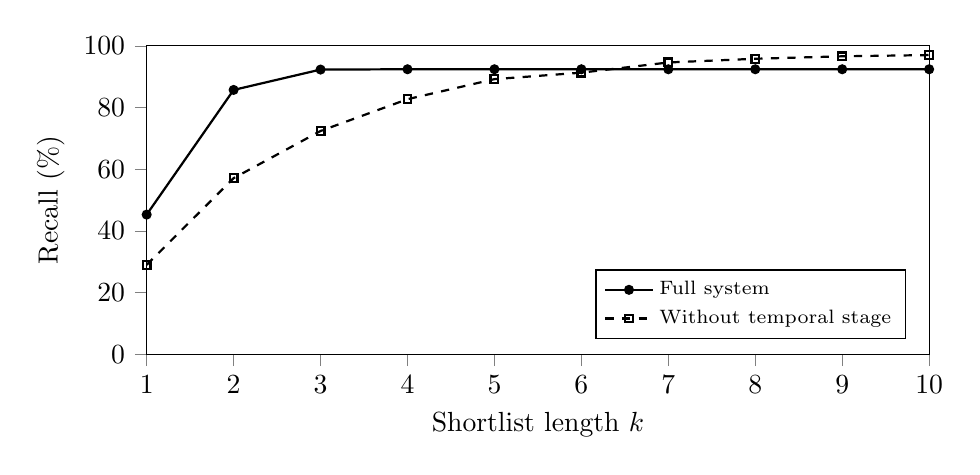
\begin{tikzpicture}
\begin{axis}[
  width=0.95\columnwidth,
  height=5.5cm,
  xlabel={Shortlist length $k$},
  ylabel={Recall (\%)},
  xmin=1, xmax=10,
  ymin=0, ymax=100,
  xtick={1,2,3,4,5,6,7,8,9,10},
  ytick={0,20,40,60,80,100},
  tick align=outside,
  tick pos=left,
  legend style={at={(0.97,0.05)},anchor=south east,font=\scriptsize,draw=black},
  legend cell align=left,
  every axis plot/.append style={line width=0.8pt,black},
]
\addplot[mark=*,mark size=1.4pt] coordinates {
  (1,45.3) (2,85.7) (3,92.3) (4,92.4) (5,92.4) (6,92.4) (7,92.4) (8,92.4) (9,92.4) (10,92.4)
};
\addlegendentry{Full system}
\addplot[dashed,mark=square,mark options={solid},mark size=1.4pt] coordinates {
  (1,29.0) (2,57.1) (3,72.4) (4,82.7) (5,89.2) (6,91.3) (7,94.6) (8,95.8) (9,96.6) (10,97.0)
};
\addlegendentry{Without temporal stage}
\end{axis}
\end{tikzpicture}
\caption{Recall against shortlist length (360 frames, 739 people).}
\label{fig:recall}
\end{figure}

Persistence lifts people above short-lived clutter, so recall@3 rises from 72.4\% to 92.3\% (Fig.~\ref{fig:recall}). The cost is the warm-up: nothing is shown in the first 4 frames, so the full system plateaus at 92.4\% and the run without tracking overtakes it for $k \geq 7$. Most frames contain 2--3 people, so recall@1 cannot exceed about 45\%.

\begin{figure}[!t]
\centering
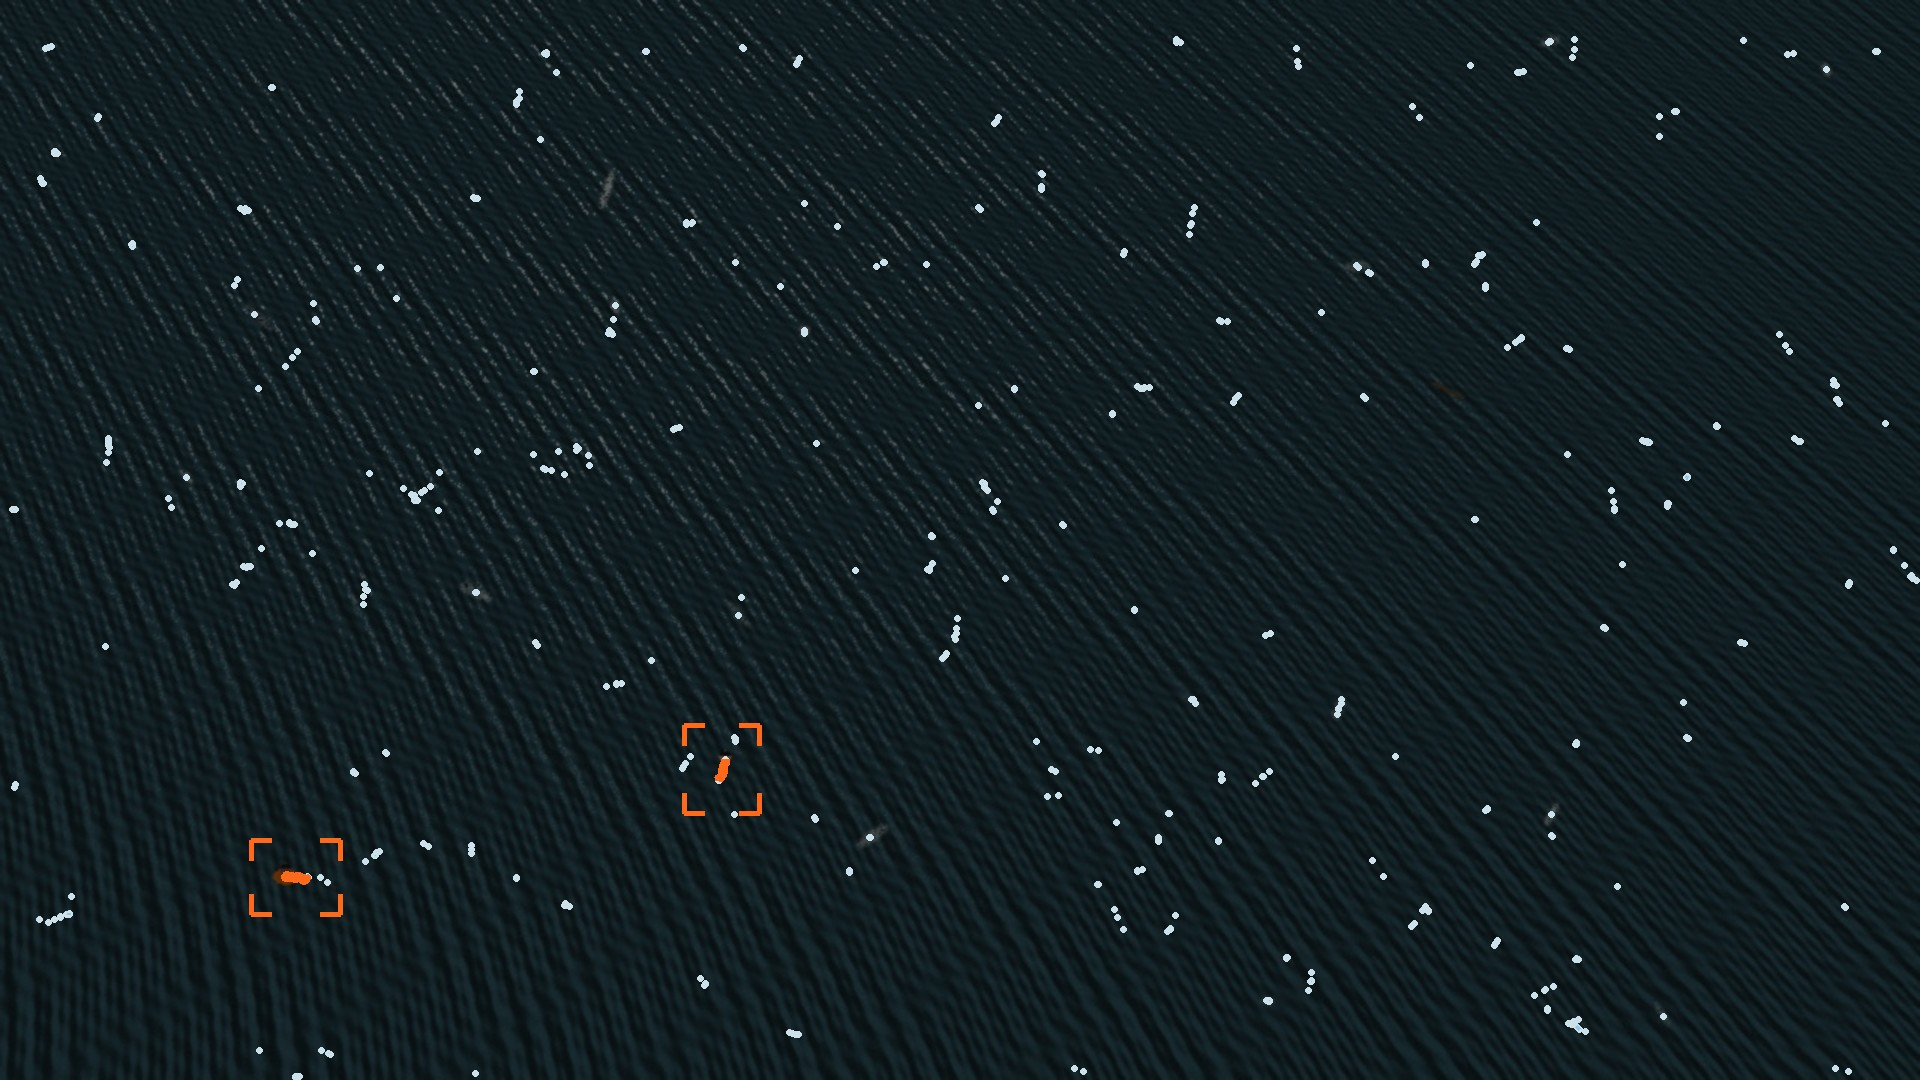
\includegraphics[width=\columnwidth]{tracks_final.jpg}
\caption{All detections across 60 frames of sequence 5. The two people form continuous tracks (orange); other detections appear briefly (pale dots).}
\label{fig:tracks}
\end{figure}

Fig.~\ref{fig:tracks} shows why tracking works: sequence 5 produced 665 raw detections, yet each person stayed on the shortlist for 56 frames and no other track lasted more than 7. Recall@5 was stable across altitude (93.2\% below 60 m, 92.9\% at 60--100 m, 89.0\% at 100--140 m, 93.3\% at 140 m and above) and target size (92.2\% under 16 px, $n=618$; 93.4\% for 16--32 px, $n=121$). Of 11 false alarms inspected at frame 31 across the six sequences, 3 resembled debris, 3 whitecaps and 5 showed nothing visible.

% ============================================================ limitations and conclusion
\section{Limitations}

\begin{itemize}
  \item Results are synthetic only; loaders are ready for SeaDronesSee~\cite{seadronessee}, MOBDrone~\cite{mobdrone} and AFO~\cite{afo}.
  \item Dark, colourless targets give weak colour and texture contrast, and very bright white clothing can be removed as glint.
  \item Coastline or a large ship in a reference window can contaminate the reference.
  \item Long-lived whitecaps or debris can be promoted to a track.
  \item Phase correlation models translation only, not rotation or zoom.
  \item Parameters are hand-tuned; night and thermal imagery are out of scope.
\end{itemize}

\section{Conclusion}

Modelling the sea rather than the person lets a purely classical pipeline find small survivors without training data. Texture anomaly scoring against a robust local reference finds candidates, and colour, shape and temporal tests remove most clutter, giving 92.4\% recall@5 and 99.3\% steady-state recall on a synthetic benchmark at 1.77 false alarms per frame. Every stage is visible and tunable in both front ends. The next step is evaluation on the public SeaDronesSee, MOBDrone and AFO datasets, followed by homography-based motion compensation.

% ============================================================ references
\begin{thebibliography}{10}

\bibitem{gonzalez} R. C. Gonzalez and R. E. Woods, \emph{Digital Image Processing}, 3rd ed. Pearson Education, 2012.

\bibitem{szeliski} R. Szeliski, \emph{Computer Vision: Algorithms and Applications}. Springer, 2011.

\bibitem{sonka} M. Sonka, V. Hlavac, and R. Boyle, \emph{Digital Image Processing and Computer Vision}, India ed. Cengage Learning, 2009.

\bibitem{howse} J. Howse, P. Joshi, and M. Beyeler, \emph{OpenCV: Computer Vision Projects with Python}. Packt Publishing, 2016.

\bibitem{baggio} D. L. Baggio, S. Emami, D. M. Escriv\'a, K. Ievgen, N. Mahmood, J. Saragih, and R. Shilkrot, \emph{Mastering OpenCV 3}, 2nd ed. Packt Publishing, 2017.

\bibitem{laganiere} R. Lagani\`ere, \emph{OpenCV Computer Vision Application Programming Cookbook}, 2nd ed. Packt Publishing, 2014.

\bibitem{ojala} T. Ojala, M. Pietik\"ainen, and T. M\"aenp\"a\"a, ``Multiresolution gray-scale and rotation invariant texture classification with local binary patterns,'' \emph{IEEE Trans. Pattern Anal. Mach. Intell.}, vol.~24, no.~7, pp.~971--987, Jul. 2002, doi: 10.1109/TPAMI.2002.1017623.

\bibitem{seadronessee} L. A. Varga, B. Kiefer, M. Messmer, and A. Zell, ``SeaDronesSee: A maritime benchmark for detecting humans in open water,'' in \emph{Proc. IEEE/CVF Winter Conf. Appl. Comput. Vis. (WACV)}, 2022, pp.~2260--2270.

\bibitem{mobdrone} D. Cafarelli \emph{et al.}, ``MOBDrone: A drone video dataset for man overboard rescue,'' in \emph{Image Analysis and Processing -- ICIAP 2022}. Cham, Switzerland: Springer, 2022, pp.~633--644.

\bibitem{afo} J. G\k{a}sienica-J\'ozkowy, M. Knapik, and B. Cyganek, ``An ensemble deep learning method with optimized weights for drone-based water rescue and surveillance,'' \emph{Integr. Comput.-Aided Eng.}, vol.~28, no.~3, pp.~221--235, 2021, doi: 10.3233/ICA-210649.

\end{thebibliography}

\end{document}
